\chapter{REVISÃO DA LITERATURA}

\section{Saturação}
A saturação consiste em uma estratégia aplicada para aumentar a eficiência e o PAPR no estágio de saída de um amplificador de potência (PA) \cite{mili}. O estudo do comportamento dos PAs demonstra que a otimização de sua eficiência ocorre em regiões de alta compressão de ganho, condição esta que, por sua vez, introduz distorções no sistema. O desafio inerente a esses amplificadores é a restrição de sua região linear; quando a potência do sinal de entrada excede esse limite, o componente satura,  ocasionando o ceifamento dos picos do sinal e a consequente geração de não linearidades. Considerando que os métodos de linearização do PA muitas vezes resultam em indicadores de desempenho superiores aos exigidos por norma, cria-se uma margem de distorção utilizável. A técnica de saturação do DPD explora justamente essa margem, visando o aumento da potência média do sinal transmitido.

\begin{figure}[!htpb]
	\centering
	\caption{ESPALHAMENTO ESPECTRAL CAUSADO PELA SATURAÇÃO}
	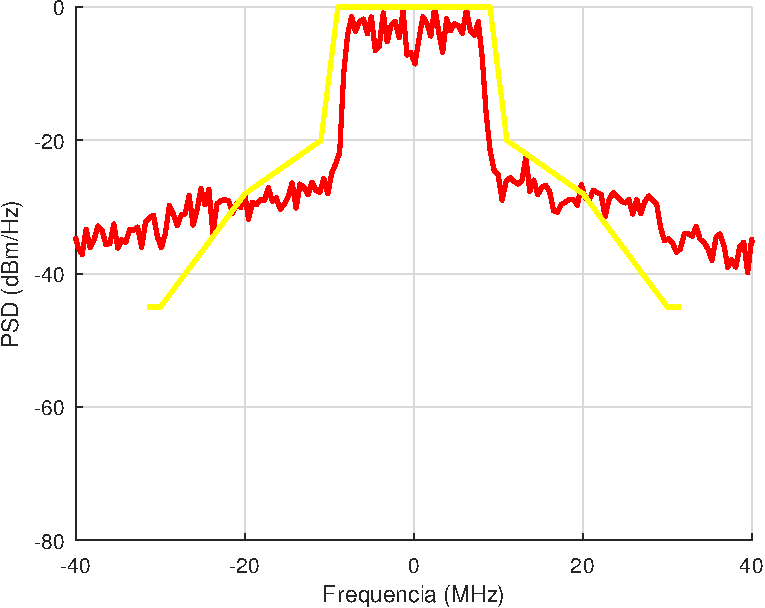
\includegraphics[width=0.75\linewidth]{fig/saturado_grafico.pdf}
	\caption*{FONTE: AUTOR}
	\label{espalhamento}
\end{figure}

\subsection{Banda única}
Na operação em banda única (1D), a modelagem da saturação é mais direta, visto que a magnitude do sinal pode ser descrita pela própria envoltória do sinal em banda base. 

\begin{equation}
	x_{c}(n) =
	\begin{cases}
		x(n), & \text{se } |x(n)| \le L \\
		L \exp j\angle x(n), & \text{se } |x(n)| > L
	\end{cases}
\end{equation}

\begin{itemize}
	\item $x(n)$: Envoltória equivalente do sinal.
	\item $L$: Nível máximo de amplitude configurado (limiar de ceifamento).
	\item $|x(n)|$: Amplitude instantânea do sinal.
	\item $\angle x(n)$: Fase instantânea do sinal.
\end{itemize}

A equação acima descreve analiticamente o mecanismo de saturação. Em cada instante discreto $n$, a amplitude instantânea do sinal é comparada ao limiar $L$. Quando o sinal se encontra dentro dessa margem operacional ($|x(n)| \le L$), sua amplitude é preservada. Por outro lado, caso a magnitude exceda esse limite, o sinal sofre ceifamento, assumindo a amplitude máxima permitida $L$. É imprescindível destacar que a fase $\angle x(n)$ é mantida, um requisito crítico para assegurar a integridade da informação modulada. 

A energia correspondente à porção ceifada do sinal é perdida e convertida em distorção não linear, modificando a forma de onda original. Contudo, a aplicação dessa técnica justifica-se pelo controle imposto ao sistema. Em vez de submeter o amplificador (PA) a picos elevados de tensão, o ceifamento preventivo assume o controle dessa compressão. Portanto, o método assegura a preservação da fase da informação, aceitando-se, como compromisso de projeto, a supressão de uma fração da energia contida na amplitude.

\subsection{Banda Dupla}
A transmissão em banda dupla (2D) é uma técnica que viabiliza a utilização de um único amplificador de potência para a transmissão simultânea de múltiplos canais em duas frequências portadoras distintas. Essa abordagem tem ganhado relevância por sua capacidade de atender às altas taxas de transmissão demandadas pelos sistemas contemporâneos, proporcionando maior eficiência espectral e energética.

O processo de saturação em banda dupla baseia-se nos mesmos princípios estabelecidos para a transmissão em banda única. Inicialmente, obtém-se a envoltória complexa equivalente, que engloba as contribuições de fase e frequência de cada portadora. O sinal resultante pode ser expresso matematicamente pela equação \cite{Artigo1}:

\begin{equation}
	x(n) = x_1(n) \exp\left( \frac{-j\Delta\omega(n-1)}{f_s} \right) + x_2(n) \exp\left( \frac{j\Delta\omega(n-1)}{f_s} \right).
\end{equation}

\noindent onde $x_1(n)$ e $x_2(n)$ representam os sinais em banda base dos dois canais, $f_1$ e $f_2$ são as frequências portadoras, e $f_s$ é a frequência de amostragem.

Após o ceifamento do sinal em um limiar $L$, aplica-se um procedimento distinto em relação à parcela excedente do sinal (a parte suprimida). Conforme abordado na seção anterior, no cenário 1D existe apenas uma portadora, de modo que a distorção gerada pelo ceifamento afeta exclusivamente aquele sinal. Na operação em banda dupla, entretanto, o cenário é mais complexo devido à presença de dois sinais modulados em frequências distintas. Nesse caso, o mero descarte da porção excedente impactaria o sinal de maneira descontrolada, podendo ocasionar intermodulação entre as bandas e a consequente perda de integridade de cada canal. Para mitigar esse problema, empregam-se técnicas de reintrodução do sinal excedente nas respectivas bandas \cite{artigo2}. 

Uma abordagem eficaz consiste na aplicação da \textbf{técnica de repartição proporcional de soma}, definida por:

\begin{equation}
	x_{ic}(n) = 
	\begin{cases}
		x_i(n), & \text{se } |x(n)| \leq L \\[6pt]
		\left( \frac{|x_i(n)| - z(n)}{2} \right) \exp(j\angle x_i(n)), & \text{se } |x(n)| > L
	\end{cases}
\end{equation}

Com a aplicação desse método, estabelece-se que, se a envoltória equivalente ultrapassar o limiar ($|x(n)| > L$), a amplitude do canal é atenuada por meio da subtração de metade do excedente ($\frac{z(n)}{2}$, em que $z(n) = |x(n)| - L$) de sua amplitude original $|x_i(n)|$. Cabe ressaltar que a fase do sinal permanece inalterada durante esse processo, resguardando as características espectrais fundamentais dos canais transmitidos. Essa estratégia viabiliza um controle mais preciso da distorção introduzida pela limitação de amplitude, conservando a qualidade de transmissão em ambas as bandas de frequência.


\begin{figure}[!htpb]
	\centering
	\caption{ENVOLTÓRIA EM BANDA DUPLA SATURADA}
	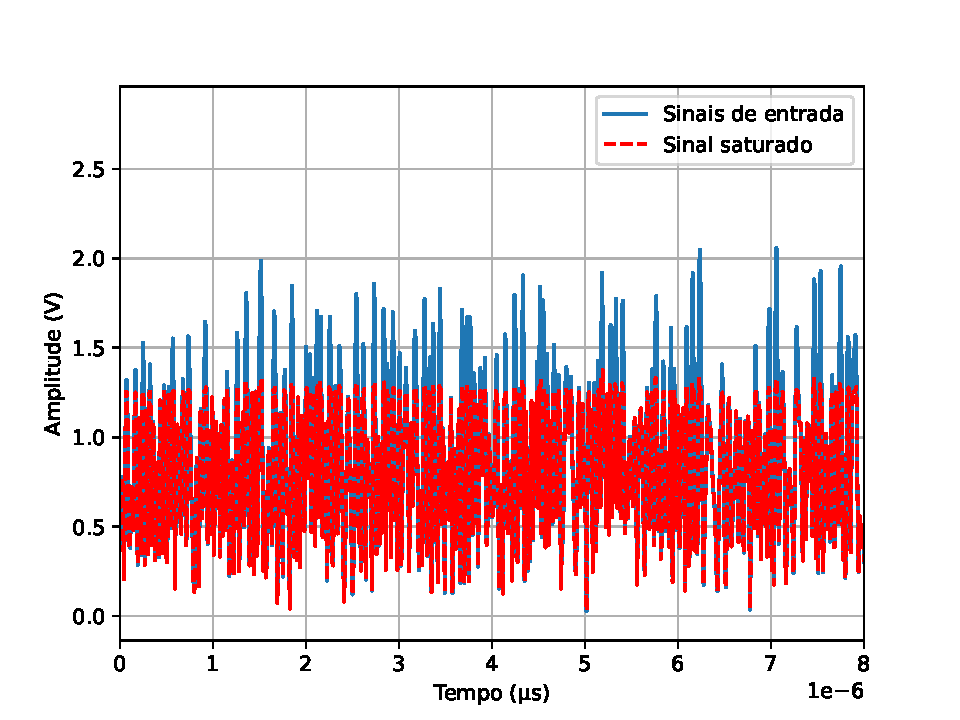
\includegraphics[width=0.75\linewidth]{fig/saturado.pdf}
	\caption*{FONTE: AUTOR}
	\label{sat}
\end{figure}

\section{Filtros FIR}
No âmbito do processamento de sinais, os filtros seletivos em frequência desempenham um papel fundamental. Esses sistemas são projetados com o propósito de permitir a passagem de componentes espectrais inseridas em um determinado intervalo, atenuando ou rejeitando as frequências fora dessa faixa. Diferentemente dos filtros analógicos, que processam sinais contínuos no tempo valendo-se de componentes eletrônicos físicos \cite{sedra2000microeletrônica}, os filtros em tempo discreto consistem em algoritmos matemáticos operando sobre sinais amostrados. Em uma cadeia de processamento digital, o sinal analógico é primeiramente amostrado e quantizado por um conversor analógico-digital (ADC). A sequência discreta resultante é então processada pelo algoritmo de filtragem, e a saída gerada pode ser reconstruída de volta ao domínio analógico por meio de um conversor digital-analógico (DAC). O cerne operacional desses filtros baseia-se em formulações matemáticas — como a operação de convolução, equações de diferenças e a transformada de Fourier —, cujas saídas dependem tipicamente da amostra de entrada atual combinada com amostras e/ou saídas anteriores \cite{oppenheim2013processamento}.

Os filtros FIR (\textit{finite impulse response}, ou resposta finita ao impulso) formam uma classe de sistemas cuja característica primordial é possuir uma resposta ao impulso $h[n]$ de duração limitada, assumindo valor nulo fora de um intervalo finito. Sua implementação recai em uma equação de diferenças linear com coeficientes constantes, o que se traduz em uma função de sistema de caráter puramente polinomial (sem polos fora da origem). A ordem do filtro é denotada por $M$, relacionando-se ao comprimento $C$ da resposta ao impulso pela equação $C = M + 1$. O projeto de um filtro FIR exige a definição prévia das especificações que ditarão seu comportamento espectral. A Figura \ref{transição} ilustra a resposta em frequência de um filtro passa-baixa prático, análogo ao abordado neste estudo. No eixo das ordenadas tem-se a magnitude da resposta, enquanto as abscissas representam a frequência normalizada no intervalo de $0$ a $\pi$. A banda de passagem delimita as frequências que devem ser preservadas; embora o comportamento ideal sugira ganho unitário e constante, sistemas práticos apresentam uma oscilação tolerável $\delta_p$, denominada \textit{ripple} de passagem. A seguir, observa-se a banda de transição, que reflete o relaxamento gradual necessário para que o filtro evolua da passagem para o bloqueio do sinal. Por fim, na banda de rejeição, objetiva-se a supressão total das componentes indesejadas; contudo, a atenuação alcançada é limitada, originando o \textit{ripple} de rejeição $\delta_r$.

\begin{figure}[!htpb]
	\centering
	\caption{TRANSIÇÃO DE UM FILTRO DIGITAL PASSA-BAIXA}
	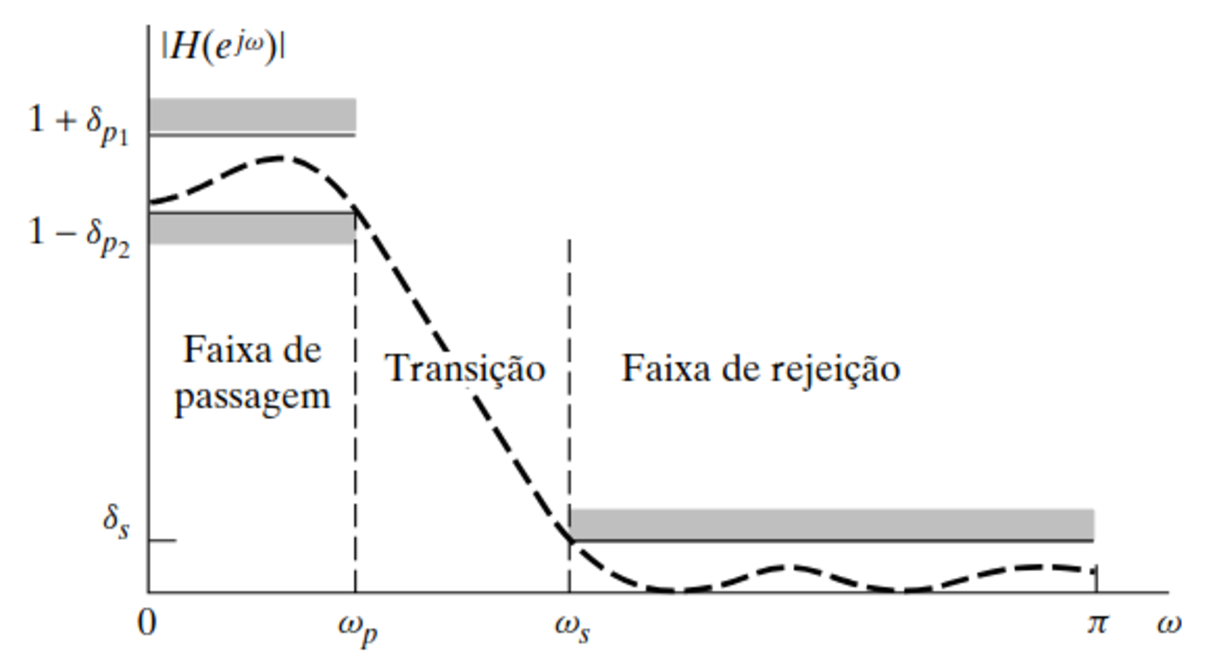
\includegraphics[width=0.75\linewidth]{fig/transição_filtro_ideal_real.pdf}
	\caption*{FONTE: \cite{oppenheim2013processamento}}
	\label{transição}
\end{figure}

\subsection{Projeto de um filtro FIR}
O procedimento adotado neste trabalho para a síntese do filtro FIR fundamentou-se no \textit{método do janelamento}. 
Essa técnica parte da especificação de uma resposta em frequência ideal, que pode ser expandida em série de Fourier de tempo discreto:

\begin{equation}
	H_d(e^{j\omega}) = \sum_{n=-\infty}^{\infty} h_d[n] \, e^{-j\omega n}
\end{equation}

A formulação expressa que a resposta em frequência ideal $H_d(e^{j\omega})$ é determinada pela combinação linear das amostras da resposta ao impulso ideal $h_d[n]$, ponderadas pelas respectivas exponenciais complexas $e^{-j\omega n}$. 
De forma complementar, a sequência $h_d[n]$ é extraída de $H_d(e^{j\omega})$ através da transformada inversa de Fourier de tempo discreto:

\begin{equation}
	h_d[n] = \frac{1}{2\pi} \int_{-\pi}^{\pi} H_d(e^{j\omega}) \, e^{j\omega n} \, d\omega
\end{equation}

Tendo em vista que sistemas fisicamente realizáveis exigem causalidade e não podem processar sequências infinitas ($n \to \pm\infty$), 
torna-se imperativo truncar a sequência $h_d[n]$. 
Esse truncamento espacial é executado pela multiplicação do sinal ideal por uma função \textit{janela} $w[n]$, resultando na resposta ao impulso do filtro projetado:

\begin{equation}
	h[n] = h_d[n] \, w[n]
\end{equation}

\noindent
Pelo teorema da convolução, essa multiplicação no domínio do tempo corresponde, no domínio da frequência, à convolução periódica entre $H_d(e^{j\omega})$ e o espectro da janela $W(e^{j\omega})$ \cite{lathi2006sinais}. 
Uma vez que $W(e^{j\omega})$ é composta por um lóbulo principal e por lóbulos laterais, o efeito direto do janelamento é o alargamento da banda de transição e a inserção de \textit{ripples} nas bandas de passagem e de rejeição.

Sob a ótica do projeto, estabelecem-se as seguintes premissas operacionais:
\begin{itemize}
	\item Janelas com maior duração no tempo $\Rightarrow$ geram lóbulos principais mais estreitos $\Rightarrow$ resultam em transições espectrais mais abruptas (menor banda de transição).
	\item Janelas com alta atenuação de lóbulos laterais $\Rightarrow$ mitigam as oscilações (\textit{ripples}) introduzidas nas bandas passante e de corte.
\end{itemize}

Por conseguinte, a seleção adequada da função janela (como Retangular, Hamming, Hann ou Blackman) traduz-se no balanço (\textit{trade-off}) técnico entre a seletividade espectral e o isolamento fora da banda de interesse.

\subsection{Ordem do filtro e número de coeficientes}
No escopo dos filtros FIR, a ordem $M$ está intrinsecamente vinculada à quantidade de coeficientes $C$ do sistema pela relação:
\[
C = M + 1
\]
O parâmetro $M$ quantifica o máximo atraso discreto introduzido pelo filtro. 
Ordens mais elevadas viabilizam transições espectrais mais abruptas e atenuações de rejeição superiores. 
Todavia, o aumento na complexidade do sistema via incremento de coeficientes resulta em impactos diretos na implementação, tais como:
\begin{itemize}
	\item \textbf{Agravamento do custo computacional:} o cálculo de cada amostra de saída demanda a execução de $C$ multiplicações e $(C-1)$ adições.
	\item \textbf{Incremento na latência intrínseca:} o atraso de grupo do filtro aumenta, exigindo cautela em aplicações com requisitos estritos de tempo real.
	\item \textbf{Maior consumo de recursos de memória:} exige-se um *buffer* mais extenso para o armazenamento dos estados anteriores da variável de entrada.
\end{itemize}

Diante exposto, a síntese do filtro FIR requer a otimização de uma função de custo implícita, buscando melhorar o desempenho espectral com a viabilidade dos recursos de *hardware* ou processamento disponíveis, modulada pela escolha criteriosa de $M$ e $w[n]$.

\subsection{Parâmetros de qualidade}
O primeiro parâmetro utilizado para analise da qualidade da implementação no sistema é o PAPR. Com essa analise a relação da potência de pico do sinal em relação a sua potência média, em termos matemáticos:

\begin{equation}
	\text{PAPR}_{\text{dB}} = 10 \cdot \log_{10} \left( \frac{\max(|x[n]|^2)}{E[|x[n]|^2]} \right)
\end{equation}

Na analise, é buscado uma diminuição do valor do PAPR, pela equação é possível perceber que a relação é inversamente proporcional ao valor da potência média, como seu aumento é o desejado, esperá-se ter uma redução do valor final, normalmente medido em decibéis.

O segundo parâmetro analisado é o de EVM, magnitude do vetor de erro, sua métrica mede a diferença entre o sinal ideal, que deveria se ter, e o sinal real. Sua visualização é dada a partir de um diagrama de constelações, uma representação visual dos símbolos de um sinal digital, Em um sistema ideal, cada ponto de dados estaria exatamente em sua posição perfeita no diagrama, mas devido a imperfeições no sistema, tais pontos se encontram em uma posição deslocada da ideal. O vetor de erro é o vetor que liga o ponto real ao seu ponto ideal correspondente.


\begin{equation}
	\text{EVM}_{\text{RMS}} = \sqrt{\frac{\frac{1}{N}\sum_{n=1}^{N}|S_{\text{real}}[n] - S_{\text{ideal}}[n]|^2}{\frac{1}{N}\sum_{n=1}^{N}|S_{\text{ideal}}[n]|^2}}
\end{equation}

O EVM leva em conta diversas imperfeições do sinal, dentre elas: Ruido de fase, distorções de amplitude e fase, vazamento de portadora. Quanto menor o valor, fica indicado que o sinal transmitido ou recebido é muito próximo do ideal. Em contrapartida, um EVM alto sugere que muitas imperfeições estão presentes no sinal, o que pode levar a erros na decodificação do mesmo.


\section{Método de Powell}
No contexto da otimização de sistemas, o método de Powell (ou método das direções conjugadas de Powell) consolida-se como uma técnica de busca direta para a minimização de funções não lineares \cite{powell1964efficient}. Sua principal vantagem reside na dispensabilidade do cálculo analítico ou numérico de derivadas. Esse aspecto é de suma importância em engenharia, especialmente quando a função custo descreve fenômenos complexos, sistemas quantizados ou rotinas de simulação que apresentam descontinuidades ou ruído acentuado, inviabilizando abordagens baseadas em gradiente, como o método de Newton-Raphson.

A base teórica do algoritmo de Powell se baseia na construção iterativa de um conjunto de direções de busca mutuamente conjugadas em relação à matriz Hessiana da função objetivo. Para um espaço de busca $n$-dimensional contendo uma função $f(\mathbf{x})$, o procedimento é inicializado a partir de uma estimativa $\mathbf{x}_0$ e de um conjunto de vetores linearmente independentes, usualmente a base ortonormal canônica $\mathbf{U} = \{\mathbf{u}_1, \dots, \mathbf{u}_n\}$. 

O ciclo iterativo do método pode ser descrito por meio da seguinte formulação:
\begin{itemize}
	\item \textbf{Minimizações sequenciais:} Iniciando em $\mathbf{p}_0 = \mathbf{x}_k$, o algoritmo executa $n$ buscas unidimensionais. Para $i = 1, \dots, n$, busca-se o escalar $\lambda_i$ que minimiza a função na direção respectiva, atualizando o ponto espacial conforme:
	\begin{equation}
		\mathbf{p}_i = \mathbf{p}_{i-1} + \lambda_i \mathbf{u}_i
	\end{equation}
	onde $\lambda_i = \arg\min_{\lambda} f(\mathbf{p}_{i-1} + \lambda \mathbf{u}_i)$.
	\item \textbf{Geração da nova direção conjugada:} Ao término da varredura direcional, o deslocamento resultante é calculado como $\mathbf{d} = \mathbf{p}_n - \mathbf{p}_0$.
	\item \textbf{Atualização da base de busca:} O conjunto de direções é reestruturado pela exclusão de uma das direções originais (tipicamente a que gerou o maior decréscimo) e pela inclusão do vetor $\mathbf{d}$, otimizando a varredura para a iteração subsequente.
\end{itemize}

A vantagem método de Powell consiste no fato de que, se aplicado a uma função quadrática de $n$ variáveis, o algoritmo alcançará o mínimo global em $n$ iterações, visto que os vetores de deslocamento $\mathbf{d}$ gerados tornam-se progressivamente conjugados.

\subsection{Aplicação do Método de Powell e Inicialização}
No contexto deste trabalho, o método de Powell foi empregado para a otimização dos coeficientes do filtro FIR inserido na malha de mitigação de distorções para sinais de banda dupla concorrente (Wi-Fi IEEE 802.11n e LTE). O objetivo principal do algoritmo de otimização consistiu em minimizar o erro entre a envoltória do sinal desejado e a envoltória efetivamente obtida após o processo de filtragem. Para orientar o algoritmo, a função de custo (função objetivo) foi definida matematicamente pelo erro quadrático em cada instante de amostragem:
\begin{equation}
	e[n] = \big( f[n] - s[n] \big)^2
\end{equation}
\noindent onde $f[n]$ representa a envoltória filtrada e $s[n]$ a envoltória saturada desejada.

Tendo em vista que algoritmos de busca direta dependem intimamente do ponto de partida para garantir uma convergência estável e evitar a estagnação em mínimos locais, a definição do vetor de busca inicial exigiu uma abordagem fundamentada nas próprias restrições físicas e normativas do sistema. O ponto de partida fornecido ao algoritmo foi estabelecido como a média aritmética das respostas ao impulso derivadas das máscaras espectrais de ambos os padrões de comunicação. 

\begin{figure}[H]
	\centering
	\caption{Mascaras da Norma}
	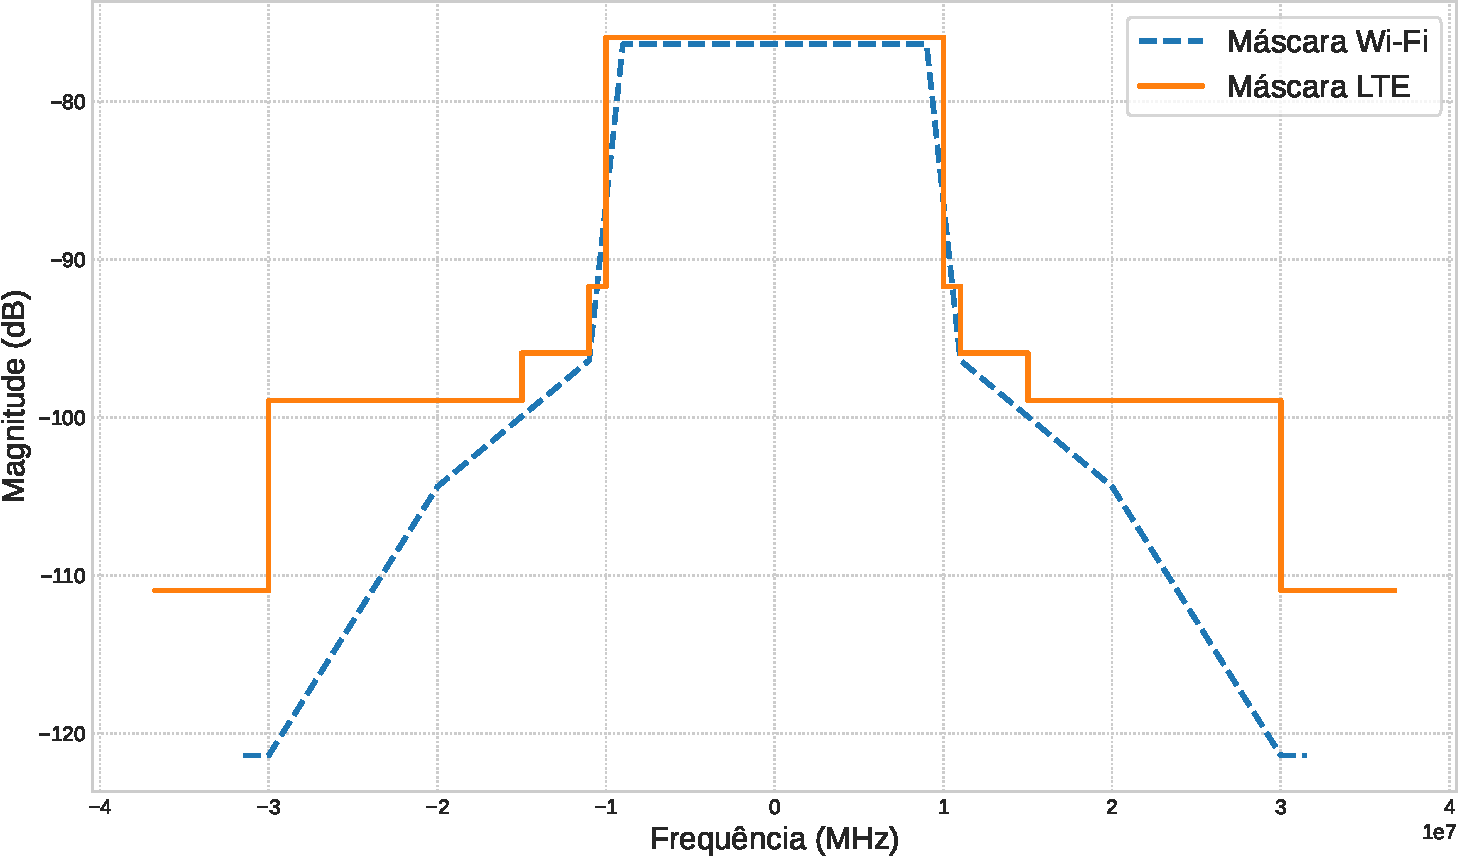
\includegraphics[width=0.75\linewidth]{fig/Máscaras_unidas.pdf}
	\caption*{FONTE: AUTOR}
	\label{fig:mascaras_unidas}
\end{figure}

Como pode ser observado na Figura \ref{fig:mascaras_unidas}, as máscaras de emissão das normas impõem limites rigorosos de espalhamento espectral (em dB). Para a extração do palpite inicial, essas máscaras foram previamente normalizadas para apresentar ganho unitário e, em seguida, mapeadas para o domínio do tempo por meio da Transformada Discreta de Fourier Inversa (IDFT), resultando nas respostas ao impulso teóricas de cada padrão. 

\begin{figure}[H]
	\centering
	\caption{Resposta ao impulso das máscaras}
	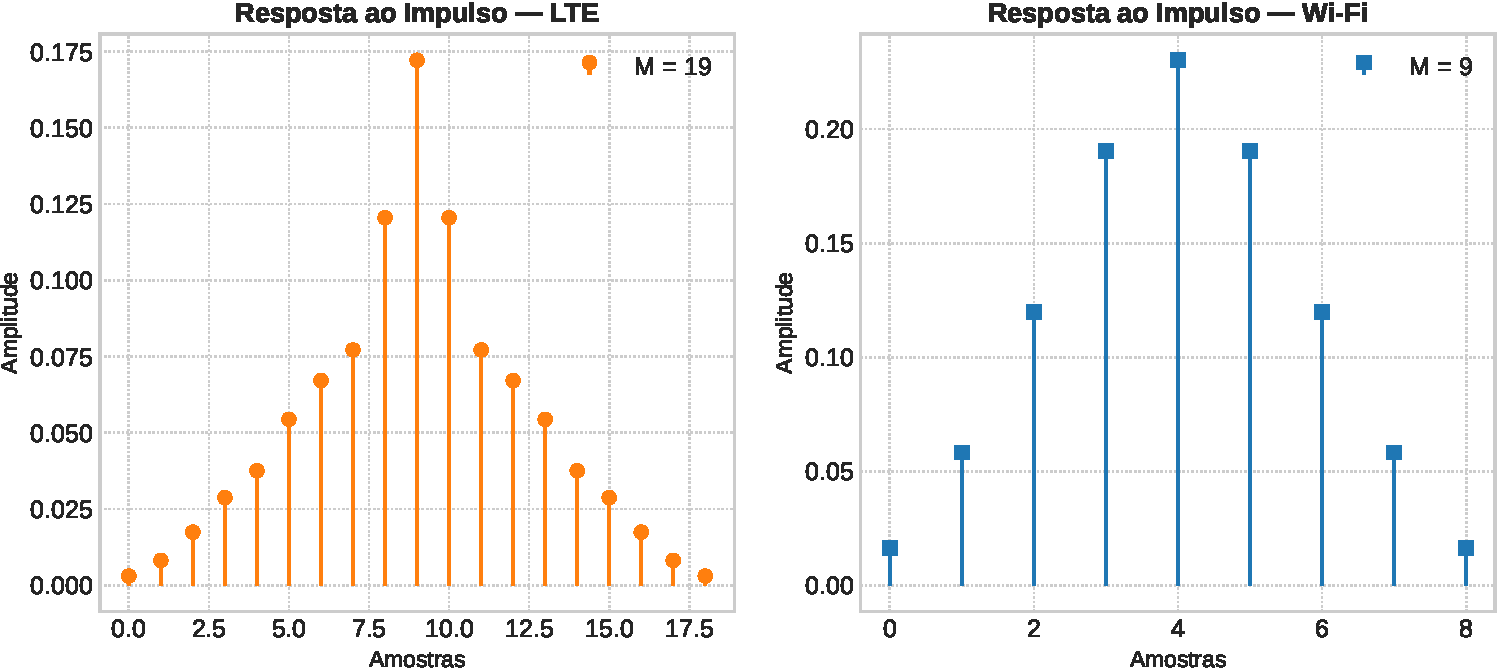
\includegraphics[width=0.75\linewidth]{fig/resposta_ao_impulso.pdf}
	\caption*{FONTE: AUTOR}
	\label{fig:mascaras_unidas}
\end{figure}

O vetor médio dessas duas respostas originou o conjunto inicial de coeficientes passado ao método de Powell, fixando desde o princípio o comprimento restrito do filtro em $C = 9$ amostras. A partir desse palpite embasado na norma, o método iterou sobre as direções de busca computando a função custo $e[n]$, ajustando o conjunto de coeficientes e preservando aqueles que demonstraram maior capacidade de supressão do erro, até que o critério de convergência fosse satisfeito.








